%% MODELO DE LATEX PARA TRABALHOS ACADÊMICOS

\documentclass[
	% -- opções da classe memoir --
	12pt,				% tamanho da fonte
	% openright,			% capítulos começam em pág ímpar (insere página vazia caso preciso)
    oneside,			% para impressão somente frente. Oposto a twoside (frente e verso)
	a4paper,			% tamanho do papel. 
	% -- opções da classe abntex2 --
	%chapter=TITLE,		% títulos de capítulos convertidos em letras maiúsculas
	%section=TITLE,		% títulos de seções convertidos em letras maiúsculas
	%subsection=TITLE,	% títulos de subseções convertidos em letras maiúsculas
	%subsubsection=TITLE,% títulos de subsubseções convertidos em letras maiúsculas
	% -- opções do pacote babel --
	english,			% idioma adicional para hifenização
	french,				% idioma adicional para hifenização
	spanish,			% idioma adicional para hifenização
	brazil,				% o último idioma é o principal do documento
	]{abntex2}


% ---
% PACOTES
% ---

% ---
% Pacotes fundamentais 
% ---
\usepackage{graphicx,url}
\usepackage{graphicx,url}

\usepackage[utf8]{inputenc}
\usepackage[brazil]{babel}
\usepackage{float}
\usepackage[utf8]{inputenc}
\usepackage[brazil]{babel}
\usepackage{float}
\usepackage{footnote}
\usepackage{graphicx}
\usepackage[most]{tcolorbox}
\usepackage{graphicx,url}
\usepackage[export]{adjustbox}
\usepackage{footnote}
\usepackage{graphicx}
\usepackage{caption}
\usepackage{subcaption}
\usepackage{graphicx}
\usepackage[most]{tcolorbox}
\usepackage{graphicx,url}
\usepackage[export]{adjustbox}
\usepackage[utf8]{inputenc}
\usepackage[brazil]{babel}
\usepackage{float}
\usepackage{footnote}
\usepackage{graphicx}
\usepackage{array}
\usepackage[most]{tcolorbox}
\usepackage{graphicx,url}
\usepackage{booktabs,chemformula}
\usepackage[export]{adjustbox}
\usepackage{longtable}
\usepackage{pdflscape}
\usepackage{graphicx}
\usepackage{float}
\usepackage{cmap}				% Mapear caracteres especiais no PDF
\usepackage{lmodern}			% Usa a fonte Latin Modern
\usepackage[T1]{fontenc}		% Selecao de codigos de fonte.
\usepackage[utf8]{inputenc}		% Codificacao do documento (conversão automática dos acentos)
\usepackage{indentfirst}		% Indenta o primeiro parágrafo de cada seção.
\usepackage{color}				% Controle das cores
\usepackage{graphicx}			% Inclusão de gráficos
\usepackage{epigraph}
\usepackage{booktabs}
\usepackage{multicol}
\usepackage[utf8]{inputenc}
\usepackage{multirow}
\usepackage{lipsum}				% para geração de dummy text
\usepackage[brazilian,hyperpageref]{backref}	 % Paginas com as citações na bibl
\usepackage[alf]{abntex2cite}



% --- 
% CONFIGURAÇÕES DE PACOTES
% --- 

% ---
% Configurações do pacote backref
% Usado sem a opção hyperpageref de backref
\renewcommand{\backrefpagesname}{Citado na(s) página(s):~}
% Texto padrão antes do número das páginas
\renewcommand{\backref}{}
% Define os textos da citação
\renewcommand*{\backrefalt}[4]{
	\ifcase #1 %
		Nenhuma citação no texto.%
	\or
		Citado na página #2.%
	\else
		Citado #1 vezes nas páginas #2.%
	\fi}%
% ---

% ---
% Informações de dados para CAPA e FOLHA DE ROSTO
% ---
\titulo{IDMATH: AJUDANDO A IDENTIFICAR CRIANÇAS COM DISCALCULIA.}
\autor{Marielsom de Araújo Rocha}
\local{Picos - PI}
\data{5 de Junho de 2017}
\instituicao{%
  Universidade Federal do Piauí
  \par
  Campus Senador Helvídio Nunes de Barros 
  \par
  Bacharelado em Sistemas de Informação}
\tipotrabalho{Relatório técnico}
% O preambulo deve conter o tipo do trabalho, o objetivo, 
% o nome da instituição e a área de concentração 
\preambulo{Trabalho de Conclusão de Curso em Bacharelado em Sistemas de Informação como requisito para a obtenção do grau de bacharel em Sistemas de Informação.}
% ---

% ---
% Configurações de aparência do PDF final

% alterando o aspecto da cor azul
\definecolor{blue}{RGB}{41,5,195}

% informações do PDF
\makeatletter
\hypersetup{
     	%pagebackref=true,
		pdftitle={\@title}, 
		pdfauthor={\@author},
    	pdfsubject={\imprimirpreambulo},
	    pdfcreator={LaTeX with abnTeX2},
		pdfkeywords={abnt}{latex}{abntex}{abntex2}{relatório técnico}, 
		colorlinks=true,       		% false: boxed links; true: colored links
    	linkcolor=blue,          	% color of internal links
    	citecolor=blue,        		% color of links to bibliography
    	filecolor=magenta,      		% color of file links
		urlcolor=blue,
		bookmarksdepth=4
}
\makeatother
% --- 


% ---
% compila o indice
% ---
\makeindex
% ---







% ----
% Início do documento
% ----
\begin{document}

% Retira espaço extra obsoleto entre as frases.
\frenchspacing 

% ----------------------------------------------------------
% ELEMENTOS PRÉ-TEXTUAIS
% ----------------------------------------------------------
% \pretextual

% ---
% Capa
% ---
\imprimircapa
% ---

% ---
% Folha de rosto
% (o * indica que haverá a ficha bibliográfica)
% ---
\imprimirfolhaderosto*
% ---






% ---
% Agradecimentos
% ---
\begin{agradecimentos}
Insira seus agradecimentos aqui.
\end{agradecimentos}
% ---

% ---
% Epigrafe
% ---
\begin{epigrafe}

\vspace*{\fill}
{ \raggedleft
	\textit{A tarefa não é tanto ver aquilo que ninguém viu, mas pensar o que ninguém ainda pensou sobre aquilo que todo mundo vê. \\
		Arthur Schopenhauer}
	~
}
\pagebreak
\end{epigrafe}

% ---
% RESUMO
% ---

% resumo na língua vernácula (obrigatório)
\begin{resumo} %% AQUI COMEÇA A PÁGINA DE RESUMO

Alguns alunos apresentam dificuldades para compreender e acompanhar as disciplinas na escola, principalmente no que diz respeito a aprendizagem da matemática, porém, é necessário observar que tais dificuldades podem não ser passageiras, tratando-se de algum transtorno de aprendizagem, como é o caso da Discalculia, que é uma dificuldade de aprendizagem referente a problemas de ordem matemática. Por conta disso, este trabalho visa apresentar uma ferramenta IDMATH, desenvolvida para auxiliar pais e profissionais da educação na realização do pré-diagnóstico em alunos que possam apresentar sinais de Discalculia em sala de aula, com idade entre 10 (dez) e 13 (treze) anos. O IDMATH possui jogos interativos e dinâmicos para efetuar o pré-diagnóstico de forma lúdica e interativa, avaliando os tipos de Discalculia de acordo com o Dr. Ladislav Kosk. Os testes foram realizados no Centro de Ensino Marcos Parente, na cidade de Picos-PI, com uma amostra de 25 (vinte e cinco) alunos do 6º ano A.
 
 % No Resumo precisa ser um pouco mais abrangente mantendo a objetividade das linhas já escritas.

 \vspace{\onelineskip}
    
 \noindent
 \textbf{Palavras-chaves}: Discalculia. Dificuldades de aprendizagem. Pré-diagnóstico.
\end{resumo} %AQUI TERMINA A PÁGINA DE RESUMO


\begin{resumo}[Abstract]

Some students have difficulties to understand and follow the disciplines in the school, mainly in what concerns the learning of the mathematics, however, it is necessary to observe that such difficulties may not be fleeting, in the case of some learning disorder, as is the case of Discalculia , Which is a learning difficulty related to mathematical problems. Therefore, this work aims to present an IDMATH tool, developed to assist parents and educational professionals in performing pre-diagnosis in students who may present signs of dyscalculia in the classroom, aged between 10 (ten) and 13 (thirteen ) years. IDMATH has interactive and dynamic games to pre-diagnose in a playful and interactive way, evaluating the types of Dysalculia according to Dr. Ladislav Kosk. The tests were carried out at the Marcos Parente Teaching Center, in the city of Picos-PI, with a sample of 25 (twenty-five) students of the 6th grade.

 \vspace{\onelineskip}
    
 \noindent
 \textbf{Key-words}: Dyscalculia. Learning difficulties. Pre-diagnosis.
 
\end{resumo}


% ---
% inserir lista de ilustrações
% ---

\listoffigures* %% o * indica que não será incluso no sumário
\cleardoublepage %% Pula página
% ---

% ---
% inserir lista de tabelas
% ---

\listoftables*
\cleardoublepage
% ---

% ---
% inserir lista de abreviaturas e siglas
% ---
\begin{siglas}
  \item[CSS] Style Sheet Cascading
  \item[CETI] Coordenação das Escolas de Tempo Integral 
  \item[HTML] Hyper Text Markup Language
  \item[IHC] Interação Humano Computador 
  \item[LEM] Língua Estrangeira Moderna
  \item[NEE] Necessidades Educacionais Especiais  
\end{siglas}
% ---

% ---
% inserir lista de símbolos
% ---


% ---
% inserir o sumario
% ---

\tableofcontents*

% ---

% ----------------------------------------------------------
% ELEMENTOS TEXTUAIS  (necessário para incluir número nas páginas)
% ----------------------------------------------------------
\textual


% ----------------------------------------------------------
% Introdução
% ----------------------------------------------------------
\chapter{Introdução} %% NOVO CAPÍTULO (REPARE QUE ELE AUTOMATICAMENTE JÁ COLOCA O NÚMERO DO CAPÍTULO E JÁ ADICIONA NO SUMÁRIO)
A aprendizagem é um fator de suma importância na vida e, cada indivíduo aprende de forma diferente. Alguns aprendem mais facilmente, já outros o esforço é um pouco maior e o educador tem o papel fundamental para identificar tal fato \cite{Spinello}.

Os profissionais da educação lidam diariamente com alunos que apresentam os mais diversos históricos escolares, principalmente no que diz respeito a escolas públicas. Dentre estes desafios enfrentados pelos educadores, encontra-se a indisciplina, problemas de ordem psicológica, comportamental e as dificuldades de aprendizagem, bastante frequentes em sala de aula \cite{Spinello}.

Para \citeonline{Correia}, as dificuldades de aprendizagem diz respeito a incapacidade para aprendizagem de leitura, escrita ou cálculos matemáticos.

Apesar de treinamentos e capacitações, os docentes não estão preparados para enfrentar estas adversidades, pois esta tarefa requer ajuda especializada de uma equipe multidisciplinar para avaliar e diagnosticar alunos que possam apresentar alguma anormalidade na escola. O aluno que sofre de algum tipo de dificuldade de aprendizagem, se não diagnosticado e tratado, tende a agravar as suas dificuldades, acarretando em evasão escolar, baixa auto-estima e outros diversos prejuízos ocasionados por problemas não identificados, diagnosticados e tratados, na escola.

É necessário fornecer ajuda para que o educador possa identificar as dificuldades que os seus alunos enfrentam, para que possam ser encaminhados para avaliação. Por conta disso, existem incontáveis teste disponíveis na internet porém não há uma base para que se encontre confiabilidade em tais testes.

Existem diversos tipos de dificuldades de aprendizagem, e dentre elas destacam-se a dislexia, a disgrafia, a dislalia, a disortografia, o Transtorno de Déficit de Atenção e Hiperatividade e a discalculia, que será abordada neste trabalho \cite{Barros}.

A partir disso, este trabalho visa apresentar uma ferramenta para o pré-diagnóstico da Discalculia, de forma que possa auxiliar os professores em sala de aula, executando o teste de maneira lúdica, através do jogos IDMATH. Desta forma é possível que o professor compreenda as dificuldades de seus alunos e assim, encaminhá-los para a equipe multidisciplinar.








\section{Contextualização do Problema}

As dificuldades de aprendizado estão cada vez mais presentes no ambiente escolar. Alguns alunos possuem certos graus de dificuldades para acompanhar e compreender determinadas disciplinas, fato bastante comum em sala de aula, principalmente no que diz respeito ao ensino e aprendizagem da matemática. A matemática, geralmente, tende a ser a disciplina com maior índice de reprovação nas escolas e, este fato nem sempre se deve a complexidade da disciplina, podendo se tratar de algum transtorno de aprendizagem, como é o caso da discalculia \cite{Almeida}

Sabe-se, no entanto, que há uma grande dificuldade na questão de identificar, diagnosticar e classificar uma dificuldade de aprendizado. Com isso, surgiu a ideia de desenvolver um aplicativo que pudesse auxiliar pais e professores a identificar a discalculia em crianças com idade de 10 (dez) a 13 (treze) anos, através do uso de jogos interativos e dinâmicos.


\section{Objetivo Geral}

Este trabalho tem como objetivo propor uma ferramenta capaz de realizar um pré-diagnóstico e classificação de alguns tipos de discalculia, de acordo com a calcificação de Kosk em 1974, em crianças com idade entre 10 e 13 anos, das series iniciais do ensino fundamental através do lúdico utilizando o jogo IDMATH. 

\section{Objetivos Específicos}

•	Apresentar  um software  que possibilite um pré-diagnóstico da discalculia;

•   sugerir uma classificação de qual possível tipo de discalculia o jogador pode apresentar de acordo com os dados obtidos; 

•   Fazer testes em escolas, com alunos na faixa etária de 10 a 13 anos.





\section{Organização do Trabalho}
Este trabalho está organizado em 6 (seis) capítulos. No capítulo 2 (dois) o Referencial Teórico, onde é apresentada a discalculia, bem como suas características, métodos de intervenção, formas de como a tecnologia pode ser uma ferramenta fundamental no diagnóstico destas crianças. No capítulo 3 (três), os trabalhos semelhantes a este. Mais adiante, no capítulo 4 (quatro) faz-se a apresentação do software, apontando seus aspectos e comportamentos. Em seguida testes e resultados no capítulo 5 (cinco) para por fim, no capítulo 6 (seis) fazermos as conclusões do trabalho e finalizando com as Referências utilizadas para o embasamento teórico da monografia. 

% ---
% Capitulo de revisão de literatura
% ---
\chapter{Referencial Teórico}



Atualmente, um dos grandes desafios para as instituições educacionais é fornecer ensino de qualidade para alunos que possuem dificuldades de aprendizagem. Apesar da ocorrência frequente no âmbito escolar, essas dificuldades são geralmente confundidas com falta de interesse do aluno \cite{Spinello}.

De acordo com \citeonline{Coelho}, os primeiros estudos realizados acerca deste assunto foram realizados por volta do século XVIII. A expressão ‘dificuldades de aprendizagem’ surgiu somente em 1962, onde suas causas eram apontadas como disfunções cerebrais, emocionais ou comportamentais. Este termo surgiu associado a obstáculos nos processos psicológicos referentes à compreensão e ao uso da linguagem, e não de problemas resultantes de deficiências motoras, sensoriais e mentais.  

Dentre as Necessidades Educativas Especiais (NEE), as dificuldades de aprendizagem representam a maior número, com 48\% de prevalência, de acordo com uma pesquisa \cite{Coelho}.
\begin{figure} [ht] 
%% hbt SIGNIFICA QUE ELE PRIMEIRO VAI TENTAR COLOCAR A IMAGEM NESTE LUGAR (h de "here"). SENÃO DER, ELE TENTA COLOCAR MAIS PRA BAIXO (b de "bottom"). SENÃO ELE COLOCA MAIS PARA CIMA (t de "top").

%% LABEL SERVE PARA VOCÊ REFERENCIAR A FIGURA NO MEIO DO TEXTO (VEJA LINHA 330: \ref{figura1}). ASSIM   VOCÊ NÃO PERDE A REFERÊNCIA QUANDO MUDA A FIGURA DE LUGAR

\caption{Grupo de NEE.}

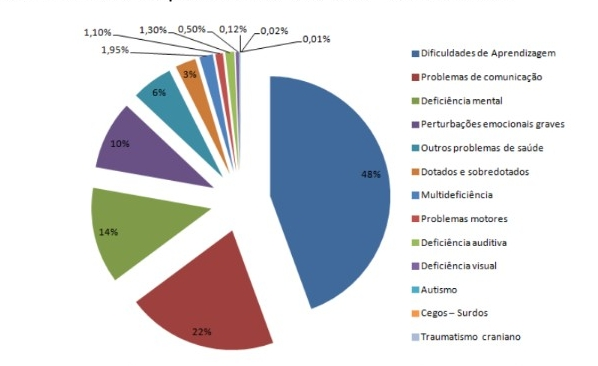
\includegraphics[width=0.72\textwidth]{graficoDA.jpg} %% PARA COLOCAR O ARQUIVO DA IMAGEM NO SHARELATEX, CLIQUE NO ÍCONE QUE PARECE UMA FLECHINHA PARA CIMA (ATUALIZAR), CLIQUE EM UPLOAD E PROCURE A IMAGEM EM SEU COMPUTADOR.
\\
\centering
\makebox{Fonte: \cite{Coelho}}
\label{matematica} 
\end{figure}


A dificuldade de aprendizagem pode se manifestar afetando a capacidade de uso da linguagem, seja ela escrita ou falada, da leitura ou até mesmo dificultando ou impossibilitando a realização de cálculos matemáticos.


Apesar de ser bastante confundida com distúrbio de aprendizagem, possui características que podem diferenciá-las. Quando se refere a distúrbio de aprendizagem, trata-se de disfunção neurológica, já quando se refere a dificuldade de aprendizagem trata-se de questões psicológicas e pode ser diagnosticada em crianças que não possuam problemas neurológicos \cite{Felipe}.


Por esse motivo, é essencial que pais e professores deem atenção aos alunos que manifestem tais dificuldades, para que lhes seja fornecido diagnóstico e acompanhamento adequado. O acompanhamento correto pode amenizar o problema, ou até mesmo levar à solução do mesmo.


Os problemas de aprendizado são diversos que vão de problemas relacionados a leitura, a escrita, até problemas matemáticos, um dos mais recorrentes em sala de aula. Estudos realizados na Universidade Católica de Brasília, mostram que cerca de 62\% dos alunos do ensino fundamental, apontam a matemática como a disciplina que encontram maiores dificuldades, Figura \ref{matematica} \cite{Machado}.


\begin{figure} [ht] 
%% hbt SIGNIFICA QUE ELE PRIMEIRO VAI TENTAR COLOCAR A IMAGEM NESTE LUGAR (h de "here"). SENÃO DER, ELE TENTA COLOCAR MAIS PRA BAIXO (b de "bottom"). SENÃO ELE COLOCA MAIS PARA CIMA (t de "top").

%% LABEL SERVE PARA VOCÊ REFERENCIAR A FIGURA NO MEIO DO TEXTO (VEJA LINHA 330: \ref{figura1}). ASSIM   VOCÊ NÃO PERDE A REFERÊNCIA QUANDO MUDA A FIGURA DE LUGAR

\caption{Disciplinas difíceis de acordo com alunos do ensino fundamental.}

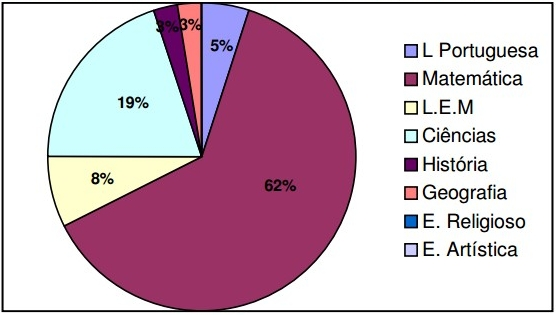
\includegraphics[width=0.68\textwidth]{grafico_pizza.jpg} %% PARA COLOCAR O ARQUIVO DA IMAGEM NO SHARELATEX, CLIQUE NO ÍCONE QUE PARECE UMA FLECHINHA PARA CIMA (ATUALIZAR), CLIQUE EM UPLOAD E PROCURE A IMAGEM EM SEU COMPUTADOR.
\\
\centering
\makebox{Fonte: \cite{Machado}}
\label{matematica} 
\end{figure}

\begin{figure} [h] 
%% hbt SIGNIFICA QUE ELE PRIMEIRO VAI TENTAR COLOCAR A IMAGEM NESTE LUGAR (h de "here"). SENÃO DER, ELE TENTA COLOCAR MAIS PRA BAIXO (b de "bottom"). SENÃO ELE COLOCA MAIS PARA CIMA (t de "top").

%% LABEL SERVE PARA VOCÊ REFERENCIAR A FIGURA NO MEIO DO TEXTO (VEJA LINHA 330: \ref{figura1}). ASSIM VOCÊ NÃO PERDE A REFERÊNCIA QUANDO MUDA A FIGURA DE LUGAR

\caption{Percentual de reprovação por disciplina.}

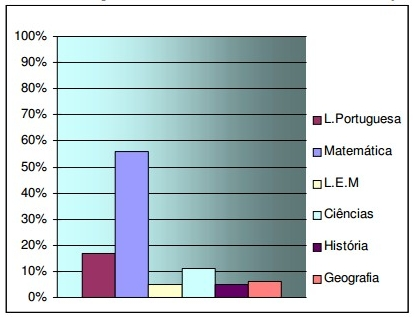
\includegraphics[width=0.60\textwidth]{grafico_barras.jpg} %% PARA COLOCAR O ARQUIVO DA IMAGEM NO SHARELATEX, CLIQUE NO ÍCONE QUE PARECE UMA FLECHINHA PARA CIMA (ATUALIZAR), CLIQUE EM UPLOAD E PROCURE A IMAGEM EM SEU COMPUTADOR.
\\
\centering
\makebox{Fonte: \cite{Machado}}
\label{reprovacao} 
\end{figure}

A matemática é uma disciplina complexa e diversos alunos não se identificam com a mesma, sendo também considerada uma das disciplinas com maior índice de reprovação, de acordo com a pesquisa foram analisados os índices de reprovação, de 18 (dezoito) alunos que se reprovaram em alguma disciplina, 10 (dez) possuem reprovação em matemática, Figura \ref{reprovacao} \cite{Machado}.







% --- Seção dentro do capítulo
\section{Discalculia}
Problemas de ordem matemática, são denominados discalculia, na qual o indivíduo apresenta dificuldades para reconhecer, manipular e efetuar cálculos matemáticos. É importante ressaltar que a discalculia não é causada por deficiência mental, déficits visuais, auditivos ou má formação escolar. O indivíduo discalcúlico possui dificuldades nas habilidades viso-espaciais, nas habilidades psicomotoras e na capacidade de reconhecer formas e tamanhos de variados objetos \cite{Almeida}.

Para \citeonline{Spinello} a Discalculia é uma má formação dos neurônio e, esse fato ocasiona na dificuldade de aprender os números matemáticos, não implicando em falta de inteligência do aluno mas, sim uma dificuldade em relação a matemática.

A palavra discalculia é uma junção dos termos "dis"  (dificuldade, desvio) e "calculare" (calcular), ou seja, é uma dificuldade de aprendizagem que interfere na capacidade do indivíduo de efetuar cálculos matemáticos \cite{Santos}.

A habilidade de aprender a matemática é encarada por muitos como uma tarefa difícil, porém esta dificuldade é ainda maior para indivíduos que possuem discalculia. A dificuldade de aprendizagem relacionada a matemática está ligada ao desenvolvimento de habilidades que necessitam do uso do conhecimento matemático \cite{Araman}.

Além da Discalculia, há também a acalculia e, geralmente há uma confusão no uso destes dois termos porém, estes possuem características que os diferenciam. A Discalculia, por sua vez, refere-se a uma desordem estrutural das capacidades matemáticas, não havendo desordens nas funções mentais generalizadas. Nesta o indivíduo possui alteração na capacidade de calcular e de manejar números. Já a segunda, a acalculia, há uma perda na capacidade de realizar cálculos e desenvolver raciocínio aritmético, há também alterações ocasionadas por conta de disfunções no sistema nervoso, manifestando-se após alguma lesão cerebral \cite{Santos}. Essas diferenças podem ser observadas através da Tabela \ref{diferencas}.

\begin{table}[h]
\caption{Diferenças entre discalculia e acalculia}
\begin{tabular}{|l|l|l}
\hline
 Acalculia & Discalculia \\ \hline
  Adquirido após lesão cerebral; & Não é causada por lesões cerebrais;  \\ \hline
  Se subdivide em acalculia primária & Associada a estudantes que apresentam dificuldades\\ 
  e acalculia secundária;  & durante a aprendizagem da matemática; \\ \hline
  Termo geralmente utilizado no caso & Desordem estrutural da maturação das capacidades \\
  de adultos; &  matemáticas; \\ \hline
  Vai desde a falta de habilidade para & Processo evolutivo e não lesional. \\
  reconhecer números até a dificuldade & \\ 
  para operá-los. & \\ \hline
\end{tabular}
\label{diferencas} 
\centering
\makebox{Fonte: \cite{Araman}}
\end{table}

Não há uma causa única para que se possa explicar a discalculia, pois tais dificuldades estão atreladas a diversos fatores. Estudos apontam que esta dificuldade pode ser ocasionada por fatores que abrangem diversas área de estudos, como a neurologia, a psicologia, a linguística, genética e a pedagogia.

De acordo com \citeonline{Lent}, o cálculo mental matemático é uma atividade de responsabilidade do hemisfério esquerdo, já o hemisfério direito é responsável pela detecção de relações espaciais quantitativas, de forma específica, no que diz respeito as relações de distância, além disso, há uma participação do hemisfério esquerdo nessa atividade através do reconhecimento das relações espaciais e qualitativas, conforme apresentado na Figura \ref{cerebro}.


\begin{figure} [h] 
%% hbt SIGNIFICA QUE ELE PRIMEIRO VAI TENTAR COLOCAR A IMAGEM NESTE LUGAR (h de "here"). SENÃO DER, ELE TENTA COLOCAR MAIS PRA BAIXO (b de "bottom"). SENÃO ELE COLOCA MAIS PARA CIMA (t de "top").

%% LABEL SERVE PARA VOCÊ REFERENCIAR A FIGURA NO MEIO DO TEXTO (VEJA LINHA 330: \ref{figura1}). ASSIM VOCÊ NÃO PERDE A REFERÊNCIA QUANDO MUDA A FIGURA DE LUGAR

\caption{Funções diferenciadas dos hemisférios especializados.}

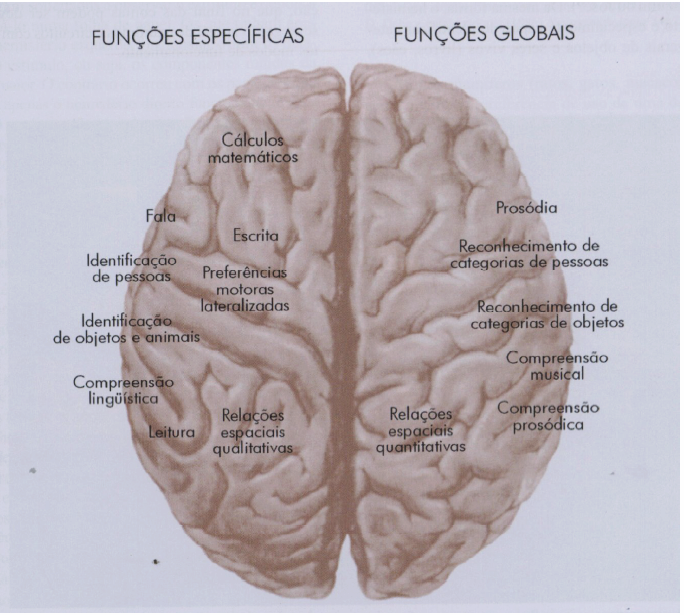
\includegraphics[width=0.62\textwidth]{cerebro.png} %% PARA COLOCAR O ARQUIVO DA IMAGEM NO SHARELATEX, CLIQUE NO ÍCONE QUE PARECE UMA FLECHINHA PARA CIMA (ATUALIZAR), CLIQUE EM UPLOAD E PROCURE A IMAGEM EM SEU COMPUTADOR.
\centering
\\
\makebox{Fonte: \cite{Lent}}
\label{cerebro} 
\end{figure}



De acordo com \citeonline{Kosk}, em sua pesquisa sobre discalculia, o autor classificou a discalculia em 6(seis) tipos distintos, que podem se manifestar no indivíduo, podendo se apresentar de forma individual ou em conjunto. Estes tipos de Discalculia são considerados até os dias atuais, sendo mencionados em diversas pesquisas e autores. Desta forma, a Discalculia é classificada em:

\begin{itemize}
    \item Discalculia verbal - se caracteriza pela dificuldade na habilidade de nomear quantidades matemáticas, números, termos e relações;
    
    \item Discalculia Practognóstica - caracteriza-se pela dificuldade de enumerar, comparar ou manipular objetos, imaginários ou reais;
    
    \item Discalculia Léxica - caracteriza-se pela dificuldade em ler símbolos matemáticos, problemas de cunho matemático;
    
    \item Discalculia Gráfica - Refere-se a dificuldade na escrita dos símbolos matemáticos;
    
    \item Discalculia Ideognóstica - refere-se a dificuldade para realizar operações mentais e para compreender os conceitos matemáticos;
    
    \item Discalculia Operacional - dificuldade para realizar operações e cálculos matemáticos.
    
\end{itemize}

É importante lembrar que a discalculia pode manifestar-se em alunos que possuem capacidades em diversas áreas, mas que apresentam dificuldades com a matemática. A criança pode não se interessar pela atividade, simplesmente por não compreendê-la.

De acordo com \citeonline{Villar}, pesquisas apontam que a discalculia acomete cerca de 4\% a 6\% da população mundial, nas pesquisas realizadas apenas com crianças. Tal porcentagem aponta a precisão de cuidados adequados, previnindo demais problemas.

% ---
% --- Seção dentro do capítulo
\section{Diagnóstico e Intervenção}

As dificuldades de aprendizagem geralmente podem ser percebidas no início da vida escolar, não decorrendo de deficiência intelectual ou de doenças adquiridas e ocasionando muito sofrimento na vida do indivíduo, principalmente nos casos não diagnosticados. Por conta disso considera-se que o diagnóstico é um fator muito importante na dificuldade de aprendizagem, pois permite que o indivíduo compreenda a razão de suas dificuldades e possa buscar ajuda especializada, a intervenção \cite{Spinello}.


O diagnóstico é realizado pela equipe multidisciplinar e envolve uma série de testes que podem qualificar ou quantificar as habilidades cognitivas do desenvolvimento escolar, tanto da fala, escrita, leitura e matemática esperado para a idade daquele aluno ou da escolarização \cite{Villar}.

A matemática é uma ferramenta essencial para o desenvolvimento do indivíduo na sociedade. Para o discalcúlico esta incapacidade acarreta em diversos prejuízos. Há alguns sinais que o indivíduo discalcúlico apresenta e que pode ser percebido pela família e professores, Tabela \ref{sinais}.
 
 % Alinhas elementos!
 
\begin{table}[ht]
\centering
\caption{Dificuldades do discalcúlico.}
\label{sinais}
\begin{tabular}{|l|l|}
\hline
 & • Visualizar conjuntos de objetos dentro de um conjunto maior;\\
& • Compreender quantidades; \\
& • Incapacidade de compreender antecessores e sucessores; \\ 
 & • Sequenciar números; \\
Dificuldades & •Classificar números;\\
& • Compreender os sinais operacionais como: +, -, x e ÷; \\ 
& • Montar operações; \\
& • Entender princípios de medida; \\
& • Lembrar sequencia de passos para realizar operações;\\
& • Problemas para diferenciar lados esquerdo e direito.\\\hline
\end{tabular}
\centering
\makebox{Fonte: \cite{Santos}}
\end{table}


É possível notar algum sinal da discalculia ainda na pré-escola porém,  é bastante cedo para um diagnóstico preciso. Somente a partir dos 7 ou 8 anos , quando a criança inicia o seu contato com os símbolos matemáticos, que é possível observar os sintomas mais visíveis \cite{Jacinto}.

Caso não haja a intervenção adequada, a defasagem de desempenho escolar pode aumentar com o passar dos anos trazendo prejuízos irreparáveis como abandono escolar, dificuldade de adaptação social e baixa autoestima \cite{Villar}.

A intervenção é realizada através de métodos pedagógicos, que podem auxiliar o discalcúlico no desenvolvimento de suas habilidades matemáticas. Os alunos com dificuldade de aprendizagem devem possuir, em seu processo de escolarização, atividades com perspectivas lúdicas, de forma que se possa garantir ensino eficaz e prazeroso para tais alunos.

De acordo com \citeonline{Santos2014}, dentre as formas de auxílio à pessoa com discalculia podemos citar:

\begin{itemize}
    \item Permitir que o aluno utilize calculadora;
    \item Não estipular tempo para as provas;
    \item Reduzir o número de questões;
    \item Permitir o acompanhamento de um tutor;
    \item Evitar avaliações orais;
    \item Optar por jogos para trabalhar as habilidades do discalcúlico;
    \item  Não desestimular o aluno.
\end{itemize}
 
\begin{center}

\begin{longtable}{@{\extracolsep{\fill}}|l|l|@{}}
\caption{Atividades de acordo com a competência.} \label{tab:long} \\
\hline %inserts double horizontal lines
   Jogo & Área de Desenvolvimento  \\ [0.5ex] 
    \hline % inserts single horizontal line
 Jogo da Memória & Motricidade fina, memória, hipótese, cores e estratégias. \\
\hline
Quebra-cabeça & \shortstack{\\ Motricidade fina e memória, formas, hipótese, análise-síntese, \\ cores, figura-fundo e estratégias.} \\
\hline
Arquiteto & Planejamento, equilíbrio, motricidade fina e estratégias. \\
\hline
Cilada & \shortstack{\\ Percepção de formas, motricidade fina, plano mental, organização, \\ encaixe, projeto e criatividade.} \\ 
\hline
Tangran & \shortstack{\\ Formas geométricas, buscas de solução, percepção de figura e formas, \\ chipótese, paciência, regras, motricidade fina e representação mental.} \\
\hline
\end{longtable}
\makebox{Fonte: \cite{Carvalho}}

\end{center}
 
As neuropsicopedagogas \citeonline{Carvalho} sugerem algumas atividades e jogos, que podem ser utilizadas na intervenção da discalculia, como pode ser observado nas Tabela \ref{competencias}:


\chapter{Trabalhos Relacionados}

%----Ferramentas semelhantes para a discalculia
O diagnóstico é um passo muito importante para indivíduos que possuem dificuldades de aprendizado, pois pode facilitar bastante a vida do mesmo. Porém, é uma tarefa difícil para os educadores identificar alguma dificuldade de aprendizado, para isso existem softwares que podem auxiliar os educadores na tarefa e, assim encaminhar os alunos para um diagnóstico efetivo, a fim de que estes adquiram o acompanhamento adequado.

Existem ferramentas computacionais que podem realizar o pré-diagnóstico, que não significa dizer que o indivíduo possua alguma disfunção mas, que este deve buscar ajuda especializada para melhor entender as suas dificuldades. Dentre estes softwares citaremos alguns semelhantes a ferramenta desenvolvida neste trabalho, apontando algumas de suas características fundamentais.

O pré-discalc é um sistema computacional, composto por 6 (seis) jogos desenvolvidos por alunos de Bacharelado em Sistemas de Informação da Universidade Federal Rural de Pernambuco (UFRPE). Este jogo tem como objetivo auxiliar profissionais da educação no pré-diagnóstico da discalculia em alunos com idade entre 10 (dez) e 12 (doze) anos. O jogo utiliza seis fases baseadas nas dificuldades dos discalcúlicos, desta forma, cada fase testa uma proficiência do jogador, em uma dificuldade específica, como: capacidade de visualizar conjuntos, entender quantidades, diferenciar lados esquerdo e direito, compreender sinais, classificar e sequenciar números \cite{Andrade}.

O EpoGames trata-se de um jogo computacional composto por 4 (quatro) jogos, que tem como objetivo capturar informações para auxiliar no processo de diagnóstico da Discalculia verbal, practognóstica, léxica e ideognóstica. Para verificar se há Discalculia no aluno, alguns dados são coletados durante as fases dos jogos e, ao final de cada uma delas é possível verificar as capacidades do aluno \cite{Medeiros}.

\begin{table}[h]
\centering
\caption{Comparação dos trabalhos semelhantes.}
\label{semelhantes}
\begin{tabular}{|c|c|c|c|}
\hline
Trabalho    & Base Teória & Resultados & Intervalo de Idade \\ \hline
Pré-discalc &   Não     &     Não      &          10-12          \\ \hline
EpoGames    &    Sim         &      Não      &         Não           \\ \hline
IDMATH      &       Sim      &    Sim        &          10-13          \\ \hline
\end{tabular}
\end{table}




%-------


\chapter{Desenvolvimento da Aplicação}

O software IDMATH foi desenvolvido através da ferramenta de desenvolvimento de jogos \textit{Construct} 2, criada pela \textit{Scirra} e tem o  intuito de ser utilizado como uma ferramenta de auxílio para pais e professores na realização do pré-diagnóstico em alunos que manifestem alguns sinais de Discalculia, em sala de aula, através de jogos dinâmicos.

O software foi desenvolvido nas seguintes etapas:

\begin{itemize}
\item Estudo bibliográfico sobre a Discalculia;
\item Conversas com a psicóloga e pedagoga da UFPI;
\item Levantamento de requisitos para construção dos jogos;
\item Desenvolvimento dos jogos;
\item Teste com crianças com idade entre 10 (dez) e 13 (treze) anos da escola Marcos Parente em Picos-PI;
\item Tabulação de dados coletados;
\item Análise dos dados coletados;
\end{itemize}

Para utilizar a ferramenta, o professor deve executar a mesma em sala de aula em forma de brincadeira, de modo a não causar desconforto na criança, ao final do jogo é possível verificar o desempenho daquele aluno, a mesma deve ser encaminhada para a equipe multidisciplinar, caso haja riscos de Discalculia.

\section{IDMATH}


A ferramenta foi desenvolvida da seguinte forma: uma tela inicial, onde o aluno irá iniciar o jogo,  este é subdividido em nove fases distintas, cada fase possui subníveis. Não é necessário que o aluno selecione as fases pois estas serão  iniciadas automaticamente.

Na tela inicial há um botão, onde o aluno poderá iniciar o jogo através de um clique e será direcionada para a Fase 01 do jogo, Figura \ref{jogo01}. Nesta, o jogador terá que identificar quantidades e efetuar cálculos matemáticos, utilizando apenas figuras. Nesta fase, o intuito é testar o desempenho do aluno no que se refere à sua capacidade de trabalhar com valores não numéricos e reconhecer quantidades, dificuldades características da Discalculia Pratognóstica, Ideognóstica e Operacional.

No decorrer das sub-fases da Fase 01, o jogador irá se deparar com diferentes quantidades de objetos e, em alguns casos terá que resolver equações para chegar a uma resposta correta. Cada sub-fase possui alternativas onde o usuário poderá escolher apenas uma como a correta.

\begin{figure} [h] 
%% hbt SIGNIFICA QUE ELE PRIMEIRO VAI TENTAR COLOCAR A IMAGEM NESTE LUGAR (h de "here"). SENÃO DER, ELE TENTA COLOCAR MAIS PRA BAIXO (b de "bottom"). SENÃO ELE COLOCA MAIS PARA CIMA (t de "top").

%% LABEL SERVE PARA VOCÊ REFERENCIAR A FIGURA NO MEIO DO TEXTO (VEJA LINHA 330: \ref{figura1}). ASSIM VOCÊ NÃO PERDE A REFERÊNCIA QUANDO MUDA A FIGURA DE LUGAR

\caption{Tela inicial  da Fase 01.}

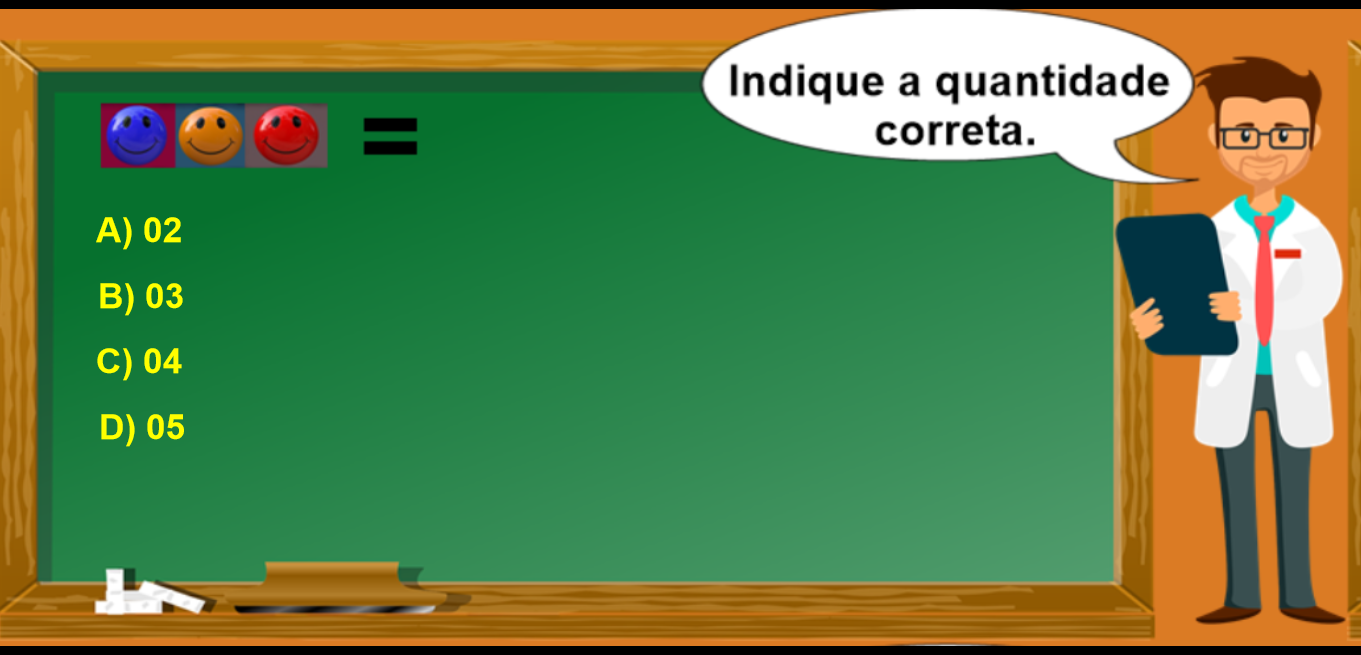
\includegraphics[width=0.62\textwidth]{jogo01.png} %% PARA COLOCAR O ARQUIVO DA IMAGEM NO SHARELATEX, CLIQUE NO ÍCONE QUE PARECE UMA FLECHINHA PARA CIMA (ATUALIZAR), CLIQUE EM UPLOAD E PROCURE A IMAGEM EM SEU COMPUTADOR.
\centering
\\
\makebox{Fonte: Autor}
\label{jogo01} 
\end{figure}


Na Fase 02 o jogador identifica conjuntos ou valores de números pares e ímpares. O objetivo dessa fase consiste em analisar o conhecimento do aluno quanto a identificação dos números pares e ímpares, o grau de dificuldade aumenta de acordo com as sub-fases seguintes Figura \ref{jogo02}. Nesta, testando dificuldades típicas da Discalculia Verbal e Pratognóstica.

\begin{figure} [h] 
%% hbt SIGNIFICA QUE ELE PRIMEIRO VAI TENTAR COLOCAR A IMAGEM NESTE LUGAR (h de "here"). SENÃO DER, ELE TENTA COLOCAR MAIS PRA BAIXO (b de "bottom"). SENÃO ELE COLOCA MAIS PARA CIMA (t de "top").

%% LABEL SERVE PARA VOCÊ REFERENCIAR A FIGURA NO MEIO DO TEXTO (VEJA LINHA 330: \ref{figura1}). ASSIM VOCÊ NÃO PERDE A REFERÊNCIA QUANDO MUDA A FIGURA DE LUGAR

\caption{Tela inicial da Fase 02.}

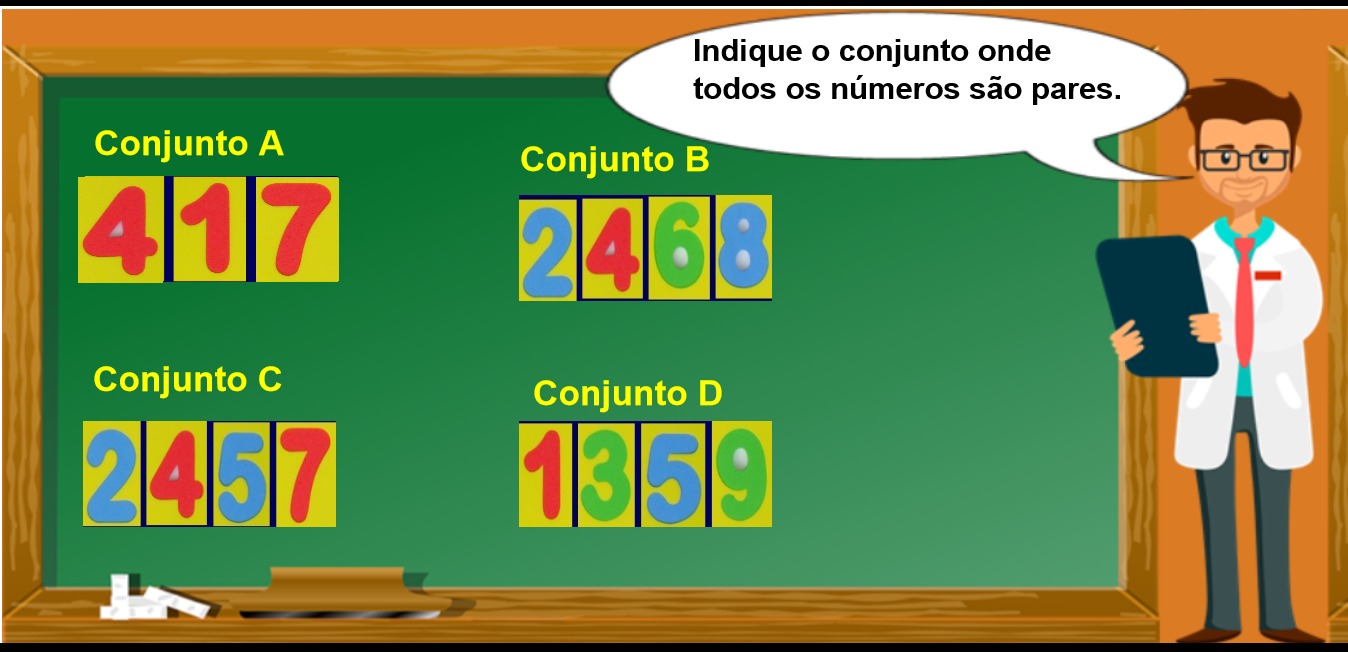
\includegraphics[width=0.62\textwidth]{jogo02.png} %% PARA COLOCAR O ARQUIVO DA IMAGEM NO SHARELATEX, CLIQUE NO ÍCONE QUE PARECE UMA FLECHINHA PARA CIMA (ATUALIZAR), CLIQUE EM UPLOAD E PROCURE A IMAGEM EM SEU COMPUTADOR.
\centering
\\
\makebox{Fonte: Autor.}
\label{jogo02} 
\end{figure}

Na Fase 03 Figura \ref{jogo03}, o jogador terá que identificar as horas em relógios analógicos. O objetivo é analisar o desempenho do aluno para identificar as horas, apenas uma alternativa é a correta e um grau de dificuldade é adicionado no decorrer das fases, como por exemplo a utilização de relógios com três ponteiros e sem numeração. Dessa forma, realizando testes referentes a Discalculia Léxica, Verbal e Pratognóstica.

\begin{figure} [ht] 
%% hbt SIGNIFICA QUE ELE PRIMEIRO VAI TENTAR COLOCAR A IMAGEM NESTE LUGAR (h de "here"). SENÃO DER, ELE TENTA COLOCAR MAIS PRA BAIXO (b de "bottom"). SENÃO ELE COLOCA MAIS PARA CIMA (t de "top").

%% LABEL SERVE PARA VOCÊ REFERENCIAR A FIGURA NO MEIO DO TEXTO (VEJA LINHA 330: \ref{figura1}). ASSIM VOCÊ NÃO PERDE A REFERÊNCIA QUANDO MUDA A FIGURA DE LUGAR

\caption{Tela inicial da Fase 03.}

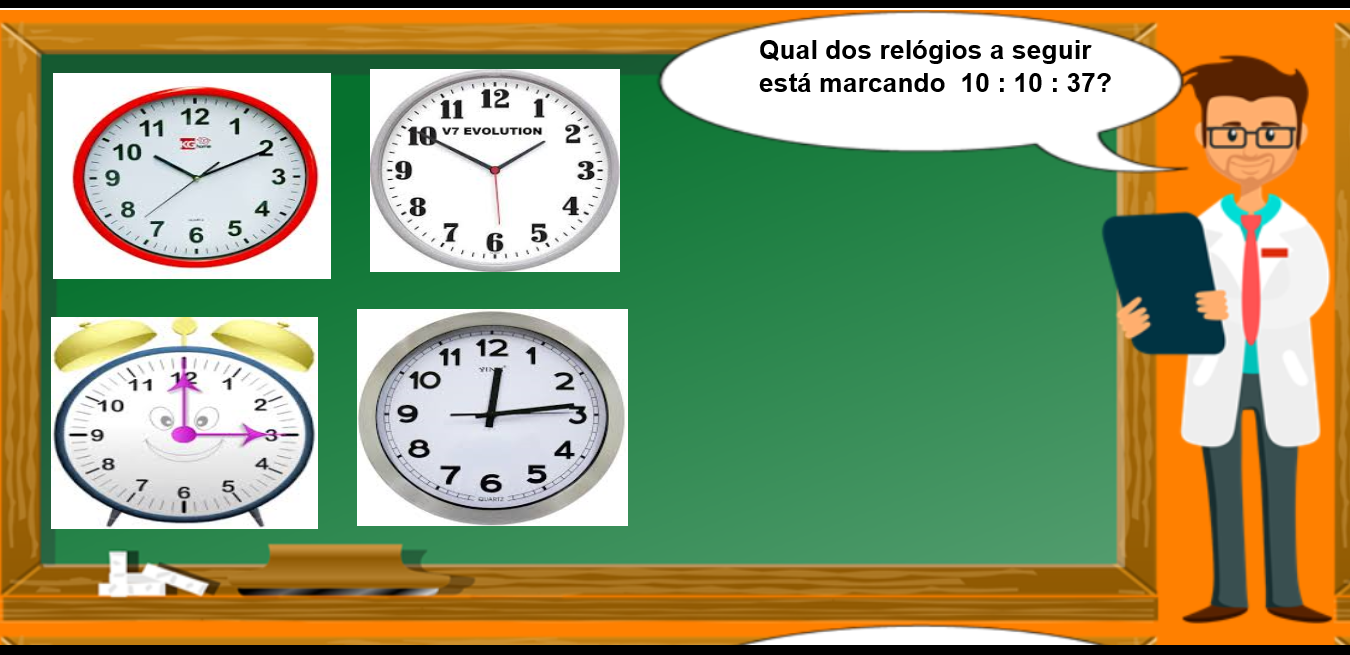
\includegraphics[width=0.62\textwidth]{jogo03.png} %% PARA COLOCAR O ARQUIVO DA IMAGEM NO SHARELATEX, CLIQUE NO ÍCONE QUE PARECE UMA FLECHINHA PARA CIMA (ATUALIZAR), CLIQUE EM UPLOAD E PROCURE A IMAGEM EM SEU COMPUTADOR.
\centering
\\
\makebox{Fonte: Autor.}
\label{jogo03} 
\end{figure}


\begin{figure} [ht] 
%% hbt SIGNIFICA QUE ELE PRIMEIRO VAI TENTAR COLOCAR A IMAGEM NESTE LUGAR (h de "here"). SENÃO DER, ELE TENTA COLOCAR MAIS PRA BAIXO (b de "bottom"). SENÃO ELE COLOCA MAIS PARA CIMA (t de "top").

%% LABEL SERVE PARA VOCÊ REFERENCIAR A FIGURA NO MEIO DO TEXTO (VEJA LINHA 330: \ref{figura1}). ASSIM VOCÊ NÃO PERDE A REFERÊNCIA QUANDO MUDA A FIGURA DE LUGAR

\caption{Tela inicial da Fase 04.}

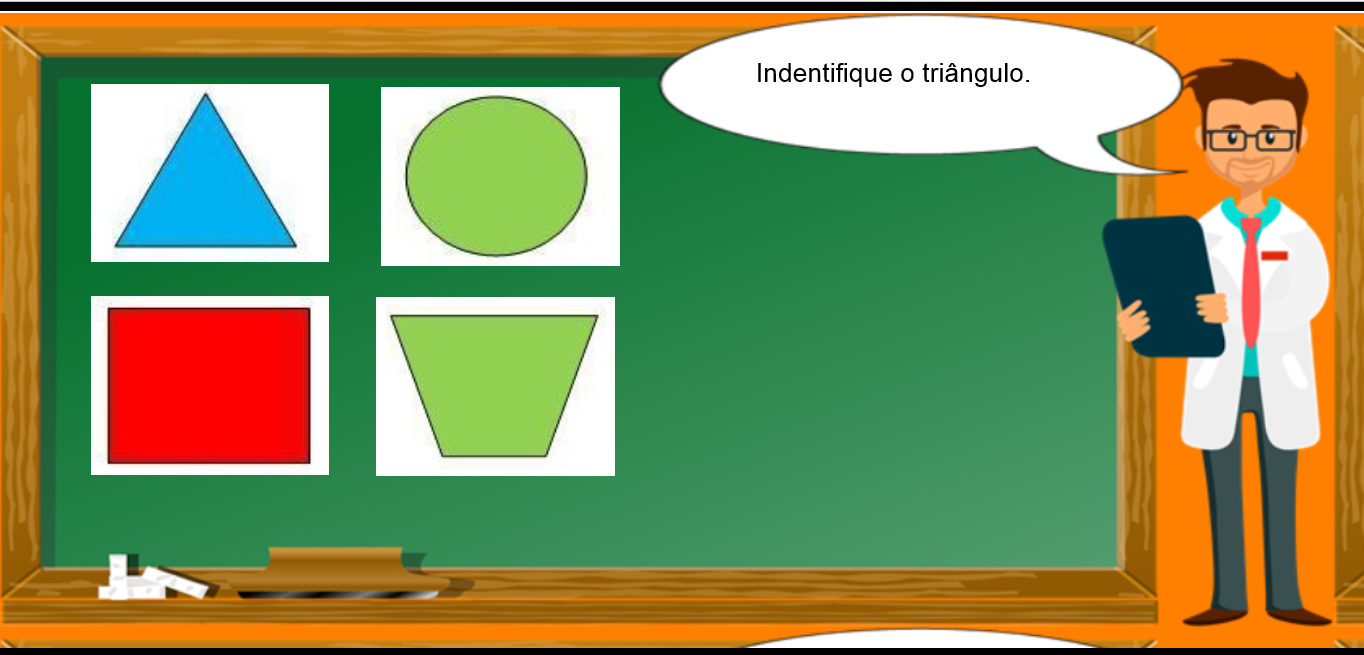
\includegraphics[width=0.62\textwidth]{jogo04.png} %% PARA COLOCAR O ARQUIVO DA IMAGEM NO SHARELATEX, CLIQUE NO ÍCONE QUE PARECE UMA FLECHINHA PARA CIMA (ATUALIZAR), CLIQUE EM UPLOAD E PROCURE A IMAGEM EM SEU COMPUTADOR.
\centering
\\
\makebox{Fonte: Autor.}
\label{jogo04} 
\end{figure}

Na Fase 04 o jogador terá que identificar figuras geométricas e números. A ideia é analisar o desempenho do aluno em relação ao reconhecimento de figuras geométricas e números, onde o aluno terá que utilizar o seu conhecimento para identificar em cada sub-fase do jogo a figura geométrica ou figura numérica Figura \ref{jogo04}. Testes referentes a Discalculia Verbal e Léxica.



Na Fase 05 o jogador terá que identificar qual o número é o maior ou menor de acordo com o que for solicitado. Esta fase tem como  finalidade analisar o desempenho do aluno para reconhecer o maior ou o menor número de acordo com o solicitado, números maiores e com valores cada vez mais próximos serão inseridos no decorrer do teste Figura \ref{jogo05}. Os testes desta fase são referentes a Discalculia Pratognóstica e Léxica.


\begin{figure} [h] 
%% hbt SIGNIFICA QUE ELE PRIMEIRO VAI TENTAR COLOCAR A IMAGEM NESTE LUGAR (h de "here"). SENÃO DER, ELE TENTA COLOCAR MAIS PRA BAIXO (b de "bottom"). SENÃO ELE COLOCA MAIS PARA CIMA (t de "top").

%% LABEL SERVE PARA VOCÊ REFERENCIAR A FIGURA NO MEIO DO TEXTO (VEJA LINHA 330: \ref{figura1}). ASSIM VOCÊ NÃO PERDE A REFERÊNCIA QUANDO MUDA A FIGURA DE LUGAR

\caption{Tela inicial da Fase 05.}

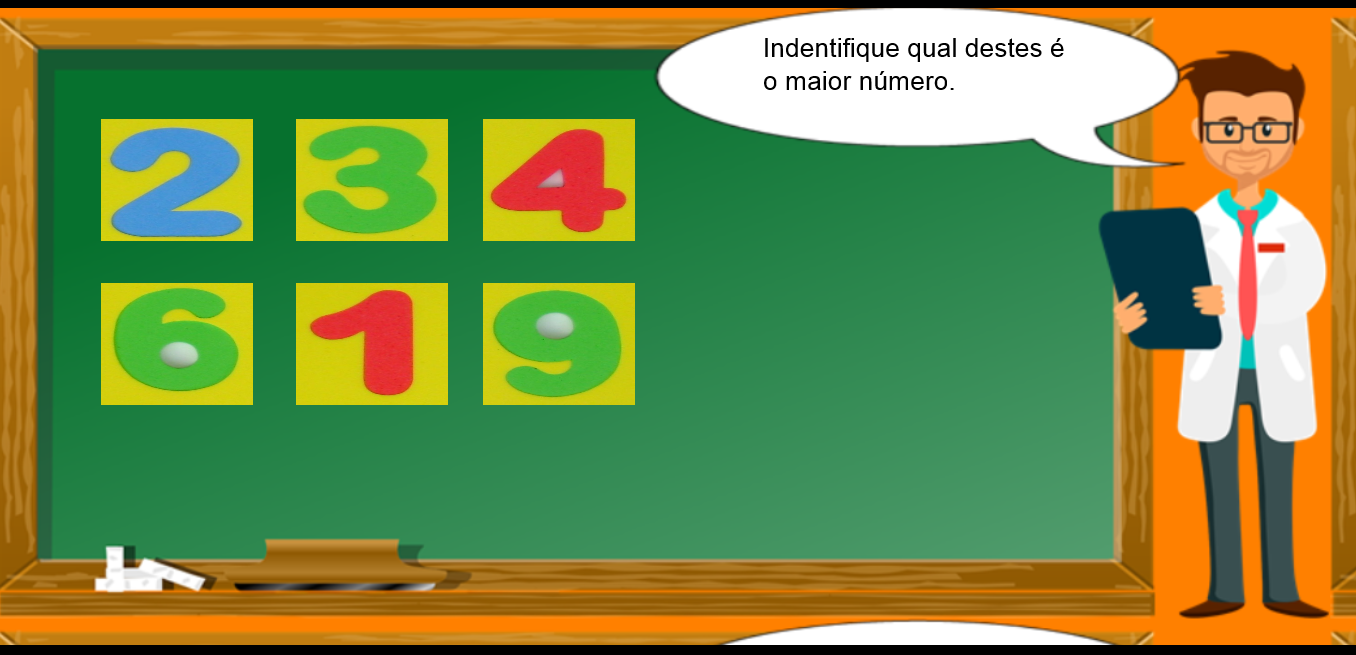
\includegraphics[width=0.62\textwidth]{jogo05.png} %% PARA COLOCAR O ARQUIVO DA IMAGEM NO SHARELATEX, CLIQUE NO ÍCONE QUE PARECE UMA FLECHINHA PARA CIMA (ATUALIZAR), CLIQUE EM UPLOAD E PROCURE A IMAGEM EM SEU COMPUTADOR.
\centering
\\
\makebox{Fonte: Autor.}
\label{jogo05} 
\end{figure}

Na Fase 06 o jogador terá que resolver alguns problemas matemáticos. O objetivo desta fase é analisar o desempenho do aluno quanto a o seu raciocínio logico na resoluções de problemas matemáticos Figura \ref{jogo06}. Nesta fase, os testes são referentes a Discalculia Pratognóstica, Ideognóstica e Operacional.

\begin{figure} [h] 
%% hbt SIGNIFICA QUE ELE PRIMEIRO VAI TENTAR COLOCAR A IMAGEM NESTE LUGAR (h de "here"). SENÃO DER, ELE TENTA COLOCAR MAIS PRA BAIXO (b de "bottom"). SENÃO ELE COLOCA MAIS PARA CIMA (t de "top").

%% LABEL SERVE PARA VOCÊ REFERENCIAR A FIGURA NO MEIO DO TEXTO (VEJA LINHA 330: \ref{figura1}). ASSIM VOCÊ NÃO PERDE A REFERÊNCIA QUANDO MUDA A FIGURA DE LUGAR

\caption{Tela inicial da Fase 06.}

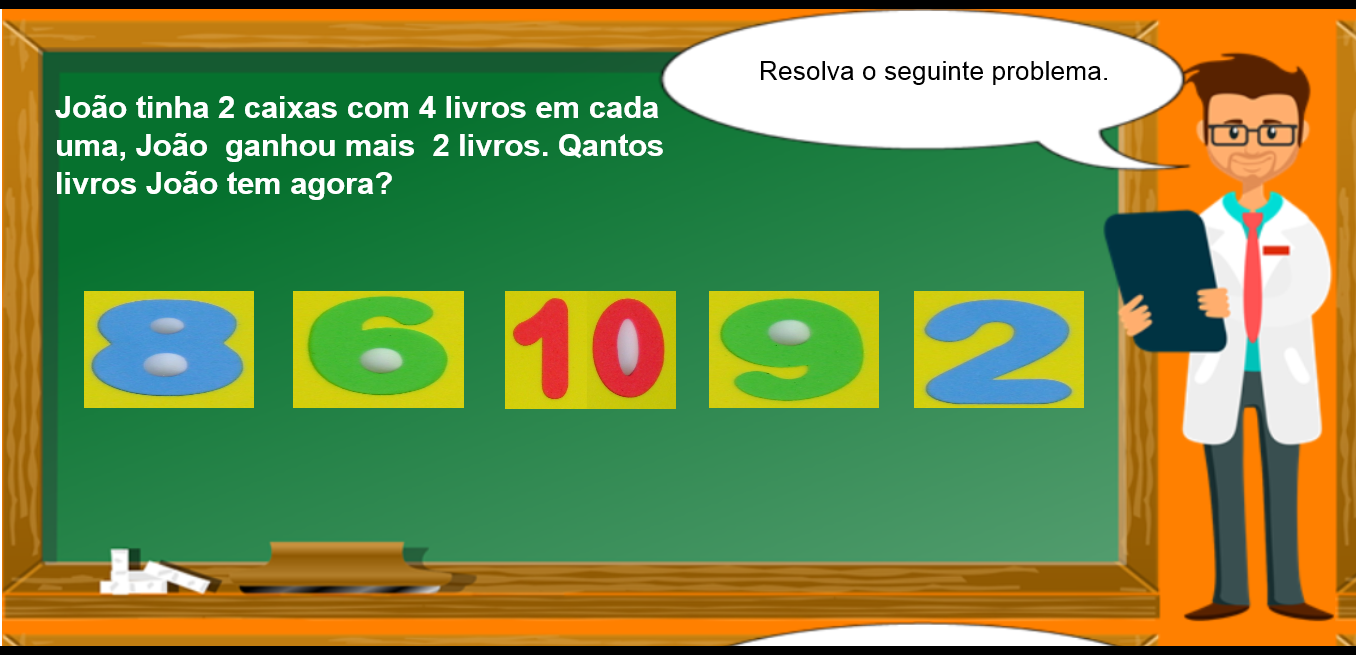
\includegraphics[width=0.62\textwidth]{jogo06.png} %% PARA COLOCAR O ARQUIVO DA IMAGEM NO SHARELATEX, CLIQUE NO ÍCONE QUE PARECE UMA FLECHINHA PARA CIMA (ATUALIZAR), CLIQUE EM UPLOAD E PROCURE A IMAGEM EM SEU COMPUTADOR.
\centering
\\
\makebox{Fonte: Autor.}
\label{jogo06} 
\end{figure}

\begin{figure} [ht] 
%% hbt SIGNIFICA QUE ELE PRIMEIRO VAI TENTAR COLOCAR A IMAGEM NESTE LUGAR (h de "here"). SENÃO DER, ELE TENTA COLOCAR MAIS PRA BAIXO (b de "bottom"). SENÃO ELE COLOCA MAIS PARA CIMA (t de "top").

%% LABEL SERVE PARA VOCÊ REFERENCIAR A FIGURA NO MEIO DO TEXTO (VEJA LINHA 330: \ref{figura1}). ASSIM VOCÊ NÃO PERDE A REFERÊNCIA QUANDO MUDA A FIGURA DE LUGAR

\caption{Tela inicial da Fase 07.}

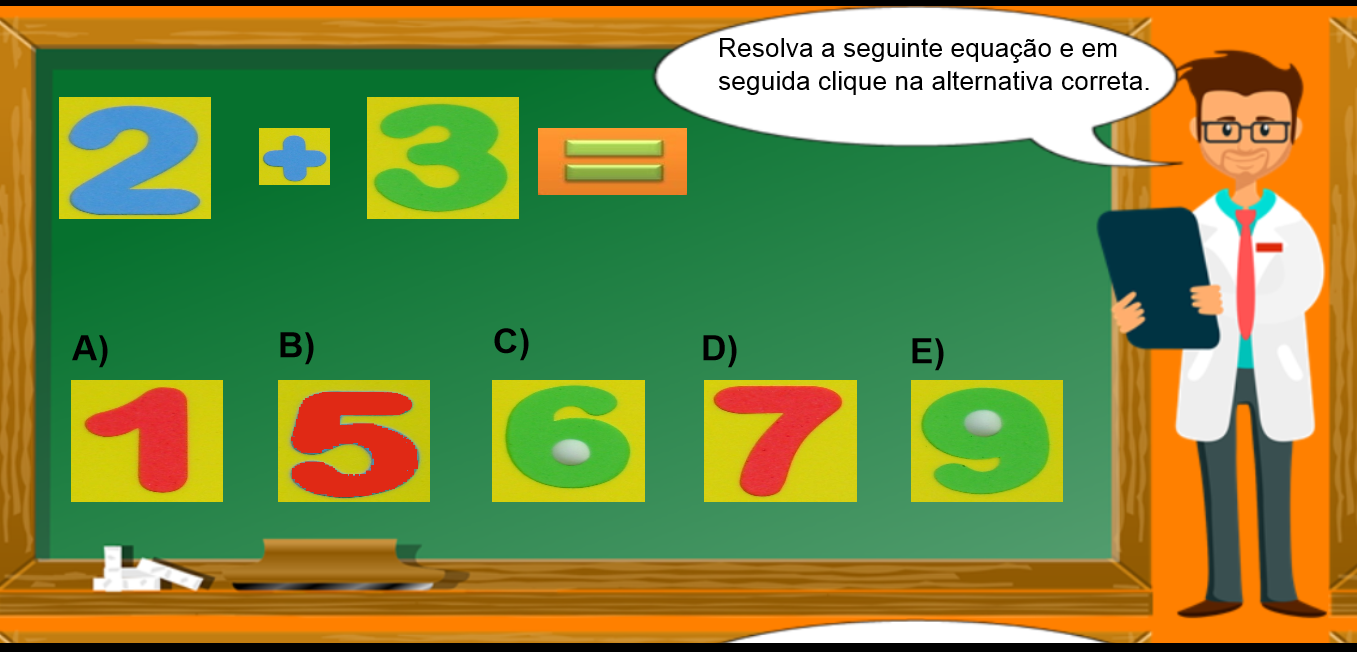
\includegraphics[width=0.62\textwidth]{jogo07.png} %% PARA COLOCAR O ARQUIVO DA IMAGEM NO SHARELATEX, CLIQUE NO ÍCONE QUE PARECE UMA FLECHINHA PARA CIMA (ATUALIZAR), CLIQUE EM UPLOAD E PROCURE A IMAGEM EM SEU COMPUTADOR.
\centering
\\
\makebox{Fonte: Autor.}
\label{jogo07} 
\end{figure}

Na Fase 07 o jogador deve resolver cálculos matemáticos utilizando apenas números. O objetivo do teste é analisar o desempenho do aluno para resolver cálculos matemáticos, a partir dos valores apresentados na tela do usuário Figura \ref{jogo07}. Nesta etapa, o teste será referente a Discalculia Ideognóstica, Operacional e Léxica.

\begin{figure} [h] 
%% hbt SIGNIFICA QUE ELE PRIMEIRO VAI TENTAR COLOCAR A IMAGEM NESTE LUGAR (h de "here"). SENÃO DER, ELE TENTA COLOCAR MAIS PRA BAIXO (b de "bottom"). SENÃO ELE COLOCA MAIS PARA CIMA (t de "top").

%% LABEL SERVE PARA VOCÊ REFERENCIAR A FIGURA NO MEIO DO TEXTO (VEJA LINHA 330: \ref{figura1}). ASSIM VOCÊ NÃO PERDE A REFERÊNCIA QUANDO MUDA A FIGURA DE LUGAR

\caption{Tela inicial da Fase 08.}

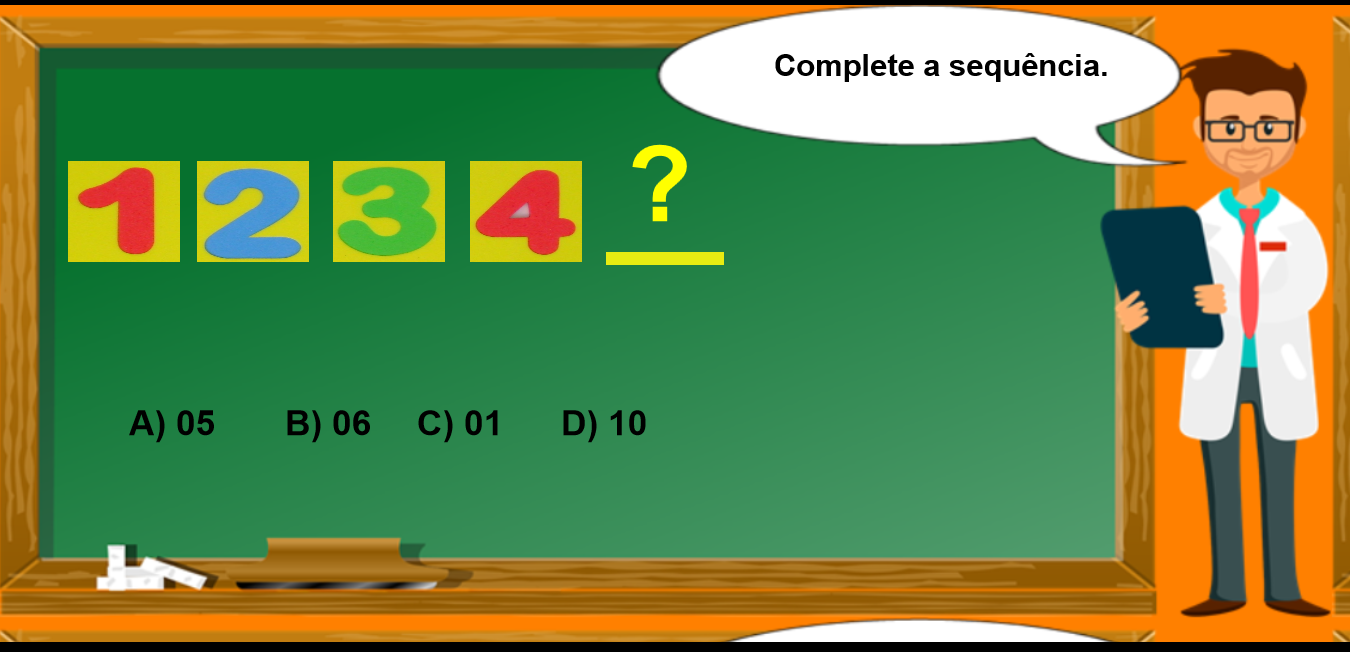
\includegraphics[width=0.62\textwidth]{jogo08.png} %% PARA COLOCAR O ARQUIVO DA IMAGEM NO SHARELATEX, CLIQUE NO ÍCONE QUE PARECE UMA FLECHINHA PARA CIMA (ATUALIZAR), CLIQUE EM UPLOAD E PROCURE A IMAGEM EM SEU COMPUTADOR.
\centering
\\
\makebox{Fonte: Autor.}
\label{jogo08} 
\end{figure}

\begin{figure} [h] 
%% hbt SIGNIFICA QUE ELE PRIMEIRO VAI TENTAR COLOCAR A IMAGEM NESTE LUGAR (h de "here"). SENÃO DER, ELE TENTA COLOCAR MAIS PRA BAIXO (b de "bottom"). SENÃO ELE COLOCA MAIS PARA CIMA (t de "top").

%% LABEL SERVE PARA VOCÊ REFERENCIAR A FIGURA NO MEIO DO TEXTO (VEJA LINHA 330: \ref{figura1}). ASSIM VOCÊ NÃO PERDE A REFERÊNCIA QUANDO MUDA A FIGURA DE LUGAR

\caption{Tela inicial da Fase 09-01.}

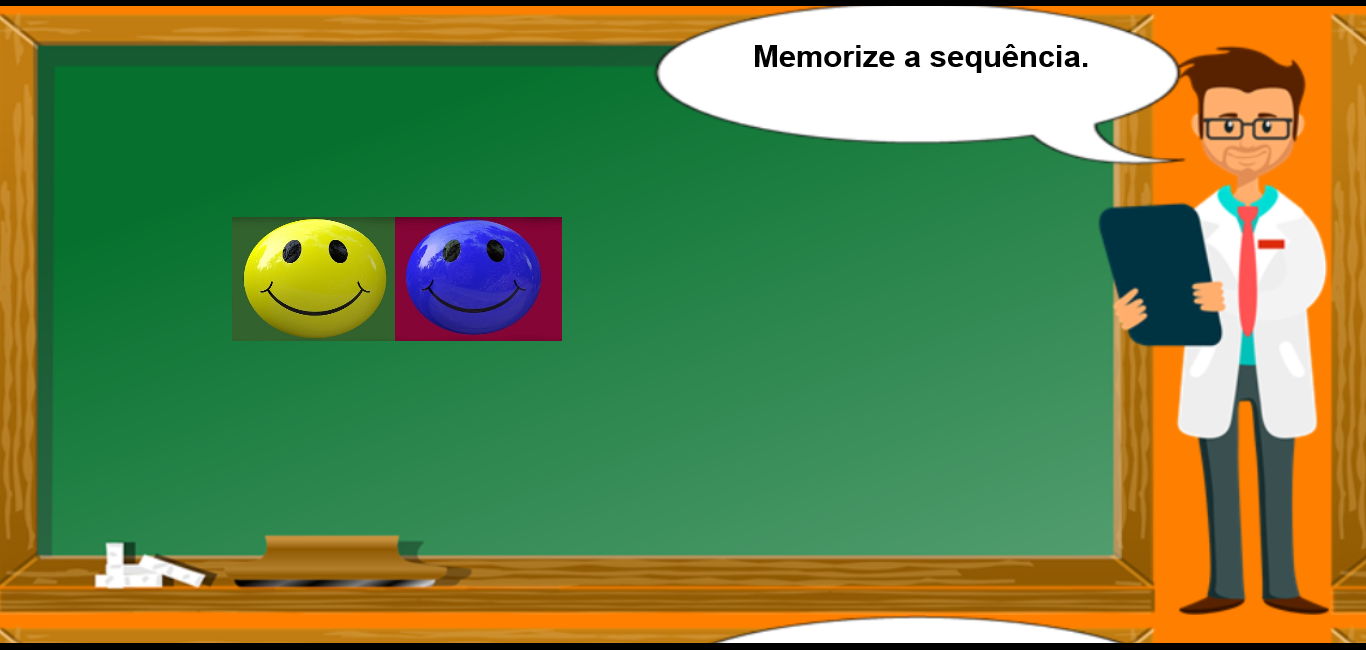
\includegraphics[width=0.62\textwidth]{jogo09_01.png} %% PARA COLOCAR O ARQUIVO DA IMAGEM NO SHARELATEX, CLIQUE NO ÍCONE QUE PARECE UMA FLECHINHA PARA CIMA (ATUALIZAR), CLIQUE EM UPLOAD E PROCURE A IMAGEM EM SEU COMPUTADOR.
\centering
\\
\makebox{Fonte: Autor.}
\label{jogo09_01} 
\end{figure}

Na Fase  08 o jogador deve completar as sequencias dos números apresentados na tela, tendo como finalidade analisar o desempenho do aluno para completar sequências numéricas simples ou espacialmente Figura \ref{jogo08}. Dessa forma, testando a Dislexia Pratognóstica e Ideognóstica. 




Na Fase 09 o jogador é submetido a um teste de memória, referente a Discalculia Ideognóstica, é aplicado da seguinte forma:
\begin{itemize}
\item Uma tela contendo imagens é apresentado por um tempo de 5 (cinco) segundo, o jogador deve memorizá-las. Logo em seguida é apresentado um layout, no qual, o jogador deve escolher uma das alternativas apresentadas Figura \ref{jogo09_01}.

\item Apos o layout de escolha ter se inicializado o jogador tem entre três opções para escolha, onde apenas uma é a opção correta, apos a seleção de uma alternativa é chamado um novo layout com uma nova sequência a ser memorizada, isso se repete ate o final da fase onde logo após o layout de desempenho do jogador é exibido Figura \ref{jogo09_02}.
\end{itemize}

\begin{figure} [h] 
%% hbt SIGNIFICA QUE ELE PRIMEIRO VAI TENTAR COLOCAR A IMAGEM NESTE LUGAR (h de "here"). SENÃO DER, ELE TENTA COLOCAR MAIS PRA BAIXO (b de "bottom"). SENÃO ELE COLOCA MAIS PARA CIMA (t de "top").

%% LABEL SERVE PARA VOCÊ REFERENCIAR A FIGURA NO MEIO DO TEXTO (VEJA LINHA 330: \ref{figura1}). ASSIM VOCÊ NÃO PERDE A REFERÊNCIA QUANDO MUDA A FIGURA DE LUGAR

\caption{Tela inicial da Fase 09-02.}

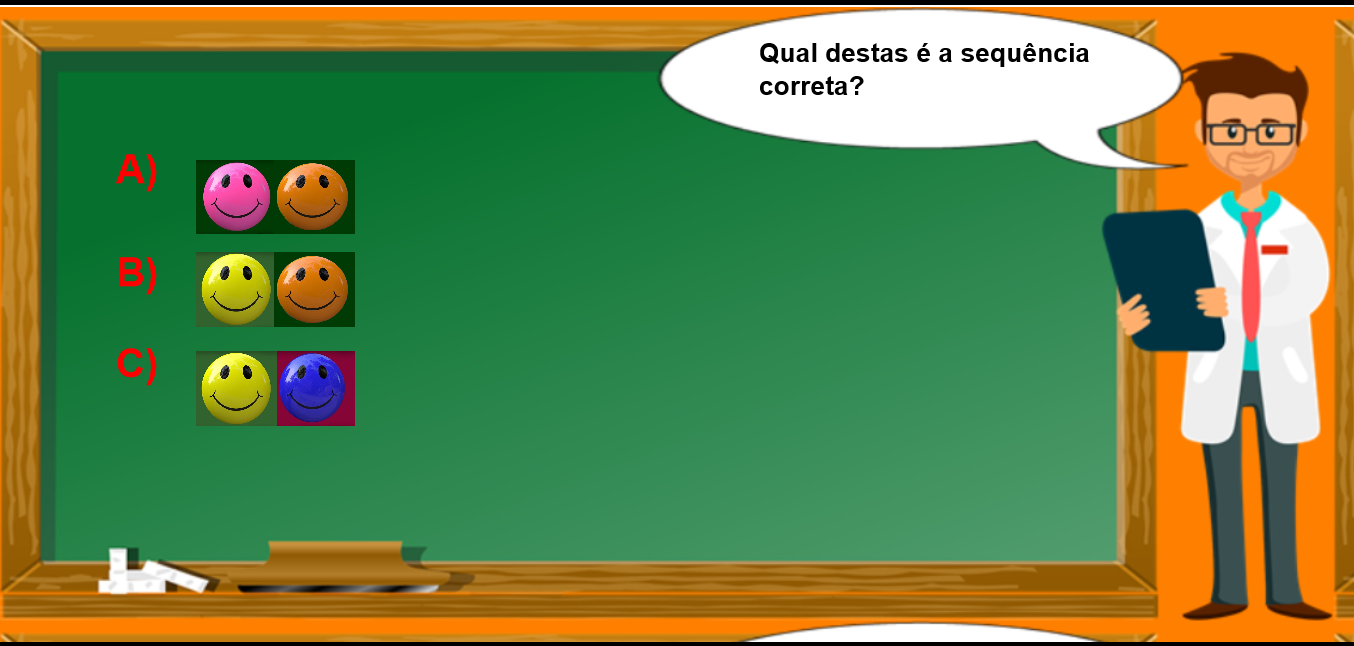
\includegraphics[width=0.62\textwidth]{jogo09_02.png} %% PARA COLOCAR O ARQUIVO DA IMAGEM NO SHARELATEX, CLIQUE NO ÍCONE QUE PARECE UMA FLECHINHA PARA CIMA (ATUALIZAR), CLIQUE EM UPLOAD E PROCURE A IMAGEM EM SEU COMPUTADOR.
\centering
\\
\makebox{Fonte: Autor.}
\label{jogo09_02}
\end{figure}



\section{Tecnologias utilizadas}

As tecnologias utilizadas para a construção desta ferramenta foram: O \textit{Construct} 2, (\textit{HyperText Markup Language}) HTML, (\textit{Style Sheet Cascading}) CSS e Java Script.

O \textit{Construct} 2, trata-se de um aplicativo construtor de jogos 2D, baseado em HTML. Esta ferramenta foi desenvolvida pela \textit{Scirra} Ltda, e lançado no ano de 2007 para desenvolvedores de jogos.

Java Script, é uma linguagem popular entre programadores para web, suportada por diversos navegadores, cria dinamismo nas páginas web. além disso, é utilizada por aplicações como Gmail e Google Maps. 

O HTML é uma linguagem de marcação de texto, desenvolvida por Tim Berners-Lee. Esta é comumente utilizada e estruturar conteúdos web, como textos e mídias. Está em sua quinta versão e tornou-se conhecido, tanto por programadores quanto por internautas.

O CSS, que surgiu com o objetivo de separar conteúdo e formato dos documentos, serve para dar cores, fontes e formatos aos elementos de uma página web. 



%---
%Testes da aplicação e resultados obtidos
%---
\chapter{Testes e Resultados}

O presente trabalho foi desenvolvido da seguinte forma, uma pesquisa bibliográfica e uma de campo sobre ferramentas computacionais utilizadas para realizar um pré-diagnostico para identificar indivíduos que possuam Discalculia. Para construção desse jogo foram utilizados os conceitos de classificação de tipos de Discalculia desenvolvidos por Kosk em 1974, assim como os principais sintomas apresentados por estes.

A pesquisa de campo foi realizada na escola CETI Marcos Parente de Picos-PI para obtenção de dados sobre a ferramenta aqui apresentada, os dados foram coletados através de um questionário com questões fechadas, para obtenção de informações válidas para avaliação do software.

O número de participantes que colaboraram voluntariamente com a pesquisa foram 25 (vinte e cinco), estes são alunos que cursam o 6º(sexto) ano A do ensino fundamental II, com idade entre 10 e 14 anos, da escola CETI Marcos Parente da cidade de Picos-PI.

Os alunos que contribuíram para a pesquisa possuem idade de acordo com o público alvo desejado para realização dos testes porém, nenhuma delas apresenta em seu histórico escolar, algum tipo de dificuldade de aprendizagem identificada, pois a escola não disponha de uma equipe multidisciplinar para realizar tais diagnósticos.

Para a coleta dos dados da pesquisa foi elaborado um questionário contendo 8 (oito) questões relacionadas a Interação Humano Computador (IHC) do jogo, cada pergunta contida no questionário tinha SIM e NÃO como opções de resposta, onde SIM era uma resposta positiva e favoráveis a usabilidade do jogo  e NÃO como opção negativa, exceto na questão 5 (cinco), onde o NÂO é algo favorável a usabilidade do jogo.

Os dados coletados foram tabulados no Excel, editor de planilhas eletrônicas da Microsoft para sistema operacional Windows, que possibilita a criação de gráficos a partir dos dados inseridos na tabela disponibilizada pelo sistema. 

A o final da pesquisa obteve-se os seguintes resultados, 83\% (oitenta e três porcento) dos alunos consultados classificaram a usabilidade do jogo como positiva, e 17\% (dezessete porcento) o classificaram com algum tipo de dificuldade para entendimento, isso pode ser observado na Tabela \ref{semelhantes}, que contém as perguntas realizadas e a quantidade de respostas obtidas para suas respectivas respostas; além do valor percentual das respostas que podem ser visualizadas no gráfico \ref{testedeihc}.



\begin{table}[h]
\centering
\caption{Resultado do teste de IHC do jogo .}
\label{semelhantes}
\begin{tabular}{|l|l|l|l|}
\hline
Questões    & SIM     & NÃO  \\ \hline
1. O usuário encontra disponíveis as informações para suas ações?    &    22     &   03   \\ \hline
2. As alternativas são legíveis?                                     &    21     &   04   \\ \hline
3. As frases são breves e objetivas?                                 &    19     &   06   \\ \hline
4. As telas apresentam somente os dados e informações necessárias?   &    22     &   03   \\ \hline
5. Você encontrou palavras difíceis?                                 &    08     &   17   \\ \hline
6. As telas são agradáveis?                                          &    23     &   02   \\ \hline
7. O jogo é fácil de usar?                                           &    24     &   01   \\ \hline
8. O jogo é de fácil compreender?                                    &    19     &   06   \\ \hline
\end{tabular}
\end{table}



\begin{figure} [h] 
%% hbt SIGNIFICA QUE ELE PRIMEIRO VAI TENTAR COLOCAR A IMAGEM NESTE LUGAR (h de "here"). SENÃO DER, ELE TENTA COLOCAR MAIS PRA BAIXO (b de "bottom"). SENÃO ELE COLOCA MAIS PARA CIMA (t de "top").

%% LABEL SERVE PARA VOCÊ REFERENCIAR A FIGURA NO MEIO DO TEXTO (VEJA LINHA 330: \ref{figura1}). ASSIM VOCÊ NÃO PERDE A REFERÊNCIA QUANDO MUDA A FIGURA DE LUGAR

\caption{Resultado do teste de IHC.}

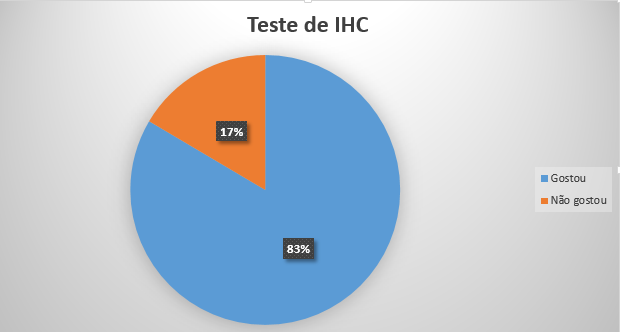
\includegraphics[width=0.62\textwidth]{testedeihc.png} %% PARA COLOCAR O ARQUIVO DA IMAGEM NO SHARELATEX, CLIQUE NO ÍCONE QUE PARECE UMA FLECHINHA PARA CIMA (ATUALIZAR), CLIQUE EM UPLOAD E PROCURE A IMAGEM EM SEU COMPUTADOR.
\centering
\\
\makebox{Fonte: Autor.}
\label{testedeihc}
\end{figure}


Os resultados de desempenho gerados pelo software, dentre os 25 ( inte e cinco) voluntários que participaram do teste apenas um dos alunos foi apontado como provável a possuir discalculia Ideognostica, que segundo \cite{Kosk} se caracteriza pela dificuldade em resolver operações mentais e na compreensão de alguns números, porem não foi possível avaliar a veracidade desta informação, por falta de uma equipe multidisciplinar para avaliar e dar um diagnostico preciso sobre o aluno. 

O percentual de erros obtido por cada aluno pode ser observado no gráfico da Figura \ref{ErrosPorAluno}, no gráfico os dados são organizados da seguinte forma, quanto maior o numero da média de erro mais provável é as chances do aluno possuir algum tipo de Discalculia.


\begin{figure} [h] 
%% hbt SIGNIFICA QUE ELE PRIMEIRO VAI TENTAR COLOCAR A IMAGEM NESTE LUGAR (h de "here"). SENÃO DER, ELE TENTA COLOCAR MAIS PRA BAIXO (b de "bottom"). SENÃO ELE COLOCA MAIS PARA CIMA (t de "top").

%% LABEL SERVE PARA VOCÊ REFERENCIAR A FIGURA NO MEIO DO TEXTO (VEJA LINHA 330: \ref{figura1}). ASSIM VOCÊ NÃO PERDE A REFERÊNCIA QUANDO MUDA A FIGURA DE LUGAR

\caption{Média de Erros Por Aluno.}

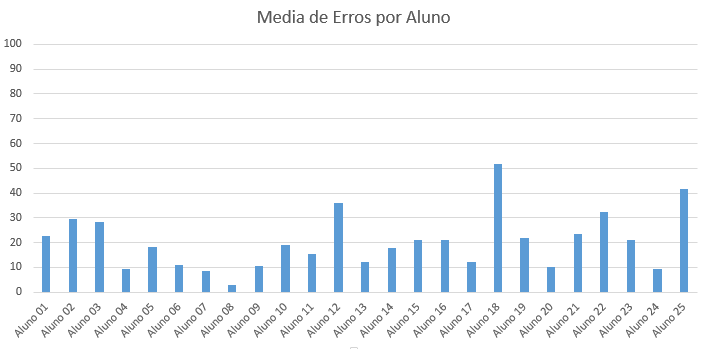
\includegraphics[width=0.70\textwidth]{ErrosPorAluno.png} %% PARA COLOCAR O ARQUIVO DA IMAGEM NO SHARELATEX, CLIQUE NO ÍCONE QUE PARECE UMA FLECHINHA PARA CIMA (ATUALIZAR), CLIQUE EM UPLOAD E PROCURE A IMAGEM EM SEU COMPUTADOR.
\centering
\\
\makebox{Fonte: Autor.}
\label{ErrosPorAluno}
\end{figure}

\section{Trabalhos Futuros}

Dentre os aprimoramentos futuros para este software, um deles é realizar testes em crianças que já tenham sido diagnosticadas com Discalculia, para que possam ser feitos aprimoramentos em sua conclusão.

Uma outra proposta futura é a implementação de um banco de dados para o armazenamento dos dados coletados durante os testes e uma tela de login, onde sera feito o cadastro da escola, a pessoa responsável pela aplicação do teste, a turma onde sera realizado e a lista de alunos que sera submetido, onde todos esses dados serão armazenados no banco de dados.

Uma outra proposta é a implementação de um sistema de inferência FUZZI para ter um resultado do pre-diagnostico mais preciso baseando-se nos dados já armazenados.

Outra ideia  de aprimoramento é inserir sons em alguns jogos, para ajudar a melhorar o pre-diagnostico de algumas das classificações de discalculia além de elaborar mais fases para que possa  ser realizado também o teste de Discalculia gráfica, tornando assim o jogo completo para analisar todos os tipos de Discalculia segundo a classificação de Kosk, além de aprimora-lo para que possa ser utilizado também em plataformas android.  



% ---
% Conclusão
% ---
\chapter{Conclusão}


Chegar ao final deste estudo sobre a Discalculia é que se pode perceber mais claramente a grande dificuldade enfrentada pelas pessoas que possuem este transtorno, professores e instituições educacionais por, muitas vezes não possuir recursos necessários para realizarem um pre-diagnósticos, identificar e de tratar estes transtornos, que se tornam cada vez mais frequentes nas escolas.

As incontáveis descobertas obtidas durante o estudo para conclusão deste trabalho impulsionaram a abertura de novos caminhos onde alguns deles foram registrados neste trabalho e que não significa o finda dos estudos, pelo contrario, deve seguir como embasamento para outros questionamentos e elaboração de novos trabalhos sobre o assunto. Existem grandes estudos relacionados a esta área e, atualmente, o auxilio das tecnologias pode ajudar estes indivíduos.

Os resultados obtidos com os testes realizados na escola com voluntários que possuíam a idade adequada a faixa etária alvo da pesquisa, mostrou-se satisfatória quanto a sua usabilidade, compreensão dos termos utilizados e resultados gerados, provendo assim uma boa base para novas pesquisas e trabalhos futuros.

O projeto foi bastante satisfatório, mesmo que, por questões cronológicas, não tenha conseguido realizar os testes com o público alvo, as crianças diagnosticadas com Discalculia. Projetar uma ferramenta para ajudar no pre-diagnostico de pessoas com Discalculia para que essas possam buscar tratamento e atividades que possam melhorar o seu desempenho, desenvolver suas abaliedades e aprimorar suas capacidades, faz com que todo o trabalho e dedicação aplicados para a realização deste projeto tenham um significado muito importante e motivacional tanto para o crescimento profissional como pessoal despertando o desejo de continuar sempre em frente e buscando sempre melhorias. 





% ----------------------------------------------------------
% ELEMENTOS PÓS-TEXTUAIS
% ----------------------------------------------------------
\postextual


% ----------------------------------------------------------
% Referências bibliográficas
% ----------------------------------------------------------
\bibliography{references} %% REFERENCIA AO ARQUIVO abntex2-modelo-references.bib

% ----------------------------------------------------------
% Glossário
% ----------------------------------------------------------
%
% Consulte o manual da classe abntex2 para orientações sobre o glossário.
%
%\glossary

% ----------------------------------------------------------
% Apêndices
% ----------------------------------------------------------

% ---
% Inicia os apêndices
% ---
\begin{apendicesenv}

% Imprime uma página indicando o início dos apêndices
\partapendices

% ----------------------------------------------------------
\chapter{Apêndice}
% ----------------------------------------------------------
Tabela de coleta de dados de usuários

1. O usuário encontra disponíveis as informações para suas ações?

( ) Sim.

( ) Não.

2. As alternativas são legíveis?

( ) Sim.

( ) Não.

3. As frases são breves e objetivas?

( ) Sim.

( ) Não.

4. As telas apresentam somente os dados e informações necessárias?

( ) Sim.

( ) Não.

5. Você encontrou palavras difíceis?

( ) Sim.

( ) Não.

6. As telas são agradáveis?

( ) Sim.

( ) Não.

7. O jogo é fácil de usar?

( ) Sim.

( ) Não.

8. O jogo é de fácil compreender?

( ) Sim.

( ) Não.


% ----------------------------------------------------------
\chapter{Apêndice}
% ----------------------------------------------------------

Teste de Discalculia


1.	Às vezes, ao copiar os números, escreve-os na ordem errada.


( ) Sim
( ) Não


2.	 Ao usar um telemóvel ou telefone escrevo os números na ordem errada. Não consigo lembrar-me de números, mesmo quando os uso regularmente.


( ) Sim
( ) Não


3.	Somar e subtrair são operações difíceis para mim.


( ) Sim
( ) Não


4.	Não consigo compreender frações.


( ) Sim
( ) Não

5.	Não compreendo o significado de números pares e ímpares


( ) Sim
( ) Não


6.	Quando alguém fala sobre números pares e ímpares tenho de pensar muito bem para identificar cada um.


( ) Sim
( ) Não


7.	Nunca poderei trabalhar numa loja porque tenho dificuldade em fazer os trocos.


( ) Sim
( ) Não


8.	Os relógios analógicos confundem-me sempre.


( ) Sim
( ) Não


9.	Nunca consegui subtrair números grandes.


( ) Sim
( ) Não


10.	Não consigo perceber a tabuada.


( ) Sim
( ) Não


11.	Não consigo identificar os símbolos matemáticos, por exemplo – ou +, às vezes não sei o seu nome ou o que cada um significa.


( ) Sim
( ) Não


12.	Todos na minha turma sabem o que à raiz quadrada, mas na realidade eu não sei.


( ) Sim
( ) Não


13.	 Acho muito difícil copiar um conjunto de números do quadro para o caderno.


( ) Sim
( ) Não


14.	Mesmo quando uso uma calculadora o resultado não está certo.


( ) Sim
( ) Não


15.	Quando tenho de resolver um problema, muitas vezes perco-me e não consigo terminar.


( ) Sim
( ) Não


16.	Às vezes esqueço-me do nome de formas geométricas como triângulo ou círculo.


( ) Sim
( ) Não


17.	Quando resolvo um exercício matemático, a folha fica sempre uma trapalhada.


( ) Sim
( ) Não


18.	Às vezes sei a resposta para um problema matemático, mas não sei explicar como lá cheguei.


( ) Sim
( ) Não


19.	Fico mesmo confuso com números elevados como 1,000 e 9,999 e não consigo identificar qual é o mais elevado.


( ) Sim
( ) Não


20.	Quando viajo não consigo perceber o valor do dinheiro dos outros países.


( ) Sim
( ) Não


21.	Não compreendo porcentagens.


( ) Sim
( ) Não


22.	 Não tenho ideia de como resolver problemas do tipo “Se um homem demora 5 minutos a percorrer 10 quilômetros, quanto tempo demora a percorrer 12?”, mesmo que outros na minha turma o consigam.


( ) Sim
( ) Não


23.	A matemática assusta-me. Na realidade não compreendo como funciona.


( ) Sim
( ) Não


24.	Algumas vezes quando tenho de responder a uma pergunta relacionada com números, não consigo lidar bem com isso e fico muito ansioso.


( ) Sim
( ) Não


% ----------------------------------------------------------
\chapter{Apêndice}
% ----------------------------------------------------------

Termo de Consentimento Livre e Esclarecimento
Baseado nas Diretrizes Contidas na Resolução CNS Nº466/2012, MS.

Eu, ................................................................., convidado(a) a participar voluntariamente do estudo experimental do trabalho intitulado “IDMATH”, recebi do graduando em Sistemas de informação pela UFPI, Campus Senador Helvídio Nunes de Barros, Marielsom de Araújo Rocha, responsável pela execução do experimento, as seguintes informações que me fez compreender sem objeções e dúvidas as seguintes informações:


	Que eu irei responder a algumas questões matemáticas contidas no jogo IDMATH, com o intuito de contribuir para obtenção dos dados necessários aos testes da nova ferramenta; 
	
	Que minha participação nesse estudo não implicará em nenhum risco à minha saúde física ou mental;
	
	Que em qualquer momento desse estudo, eu poderei me recusar à continuar participando desse estudo;
	
	Que os resultados obtidos por meio de minha participação não possibilitaram a minha identificação, exceto ao responsável por este estudo;
	
	Que o estudo realizado iniciou-se às ....:.... na data ..../..../.... e seu término às ....:.... na data ..../..../..... .

Considerando, que fui informado(a) dos objetivos e da relevância do estudo proposto, e de como será minha participação, dos procedimentos de que não há riscos decorrentes deste estudo, declaro o meu consentimento em participar da pesquisa, como também concordo que os dados obtidos por meio desse sejam utilizados para fins científicos (publicações). Estou ciente de que receberei uma via desse documento.

.................................................

Assinatura do Participante ou Responsável Legal



\end{apendicesenv}
% ---


\end{document}
